% Worksheet W4 – Research question and thesis statement (2 pages)
% Übersetzen: latexmk -xelatex ws-w4-research-question.tex
% Lösungsfassung: ws-w4-research-question-lsg.tex
% ============================================================
% ab-vorlage.tex – gemeinsame Vorlage der Arbeitsblätter
% englisch/12/w-seminar-time/arbeitsblaetter/  (W-Seminar "Time")
% Übersetzen mit:  latexmk -xelatex <datei>.tex   (oder zweimal xelatex)
% Gestaltung wie englisch/13/questions-on-the-text/arbeitsblaetter/ab-vorlage.tex,
% Antwortplatz-Makros (8-mm-Linien) wie informatik/10/java/arbeitsblaetter/ab-vorlage.tex
% Schriften: Carlito (Fließtext), Poppins (Überschriften)
% ============================================================
\documentclass[10pt,a4paper]{article}
\usepackage[a4paper,top=12mm,bottom=13mm,left=14mm,right=14mm,headsep=4mm,headheight=12pt,footskip=7mm]{geometry}
\usepackage{fontspec}
\setmainfont{Carlito}
\newfontfamily\headfont{Poppins}[UprightFont=* Medium, BoldFont=* Medium]
\newfontfamily\headlight{Poppins Light}
\usepackage{xcolor}
\definecolor{prim}{HTML}{2563EB}
\definecolor{primdark}{HTML}{1E3A8A}
\definecolor{sec}{HTML}{7C3AED}
\definecolor{dusk}{HTML}{171A3F}
\definecolor{brass}{HTML}{D9AB2F}
\definecolor{primtint}{HTML}{EFF6FF}
\definecolor{sectint}{HTML}{F5F3FF}
\definecolor{ink}{HTML}{1E293B}
\definecolor{muted}{HTML}{64748B}
\definecolor{rule}{HTML}{CBD5E1}
\definecolor{good}{HTML}{059669}
\definecolor{goodtint}{HTML}{ECFDF5}
\definecolor{warn}{HTML}{B45309}
\definecolor{warntint}{HTML}{FFFBEB}
\definecolor{bad}{HTML}{B91C1C}
\definecolor{badtint}{HTML}{FEF2F2}
% Farben der Zeit-Dimensionen (wie auf der Website)
\definecolor{dlit}{HTML}{B83280}
\definecolor{dphys}{HTML}{2563EB}
\definecolor{dcs}{HTML}{0F8F84}
\definecolor{dpsy}{HTML}{C26A06}
\definecolor{dlang}{HTML}{7C3AED}
\definecolor{dbey}{HTML}{4B5563}
\color{ink}
\usepackage[most]{tcolorbox}
\usepackage{tikz}
\usetikzlibrary{positioning,calc,arrows.meta,shapes.misc}
\usepackage{enumitem}
\setlist{nosep,leftmargin=1.1em,topsep=1pt}
\setlist[itemize]{label=\textcolor{prim}{\small\textbullet}}
\usepackage{tabularx,array,booktabs,colortbl}
\usepackage{multicol}
\usepackage{fancyhdr}
\usepackage{lastpage}
\usepackage{amssymb}
\usepackage{qrcode}
\usepackage{microtype}
\setlength{\parindent}{0pt}
\setlength{\parskip}{0pt}
\linespread{1.02}

% ---------- Kopf- und Fußzeile ----------
\newcommand{\wskopf}{W-Seminar English · Time · Year 12}
\pagestyle{fancy}
\fancyhf{}
\renewcommand{\headrulewidth}{0pt}
\fancyhead[L]{\footnotesize\headlight\textcolor{muted}{\wskopf}}
\fancyhead[R]{\ifnum\value{page}=1\footnotesize\headlight\textcolor{muted}{Name: \rule{38mm}{0.3pt}\quad Date: \rule{18mm}{0.3pt}}\fi}
\fancyfoot[L]{\scriptsize\textcolor{muted}{edu-mrh.de/englisch/12/w-seminar-time}}
\fancyfoot[R]{\scriptsize\textcolor{muted}{\thepage\,/\,\pageref*{LastPage}}}

% ---------- Titel ----------
% \wstitel{Kürzel}{Titel}{Untertitel}
\newcommand{\wstitel}[3]{%
  \begin{tcolorbox}[enhanced,colback=dusk,colframe=dusk,arc=2mm,boxrule=0pt,
     left=4mm,right=4mm,top=2.2mm,bottom=2.2mm,
     interior style={left color=dusk,right color=primdark}]
    \color{white}{\headlight\footnotesize #1}\\[0.3mm]
    {\headfont\LARGE #2}\\[0.6mm]
    {\small #3}
  \end{tcolorbox}\vspace{1mm}}

% ---------- Boxen ----------
% \begin{wsbox}[Optionen]{Nummer}{Überschrift} ... \end{wsbox}
\newtcolorbox{wsbox}[3][]{enhanced,breakable,colback=white,colframe=rule,boxrule=0.5pt,arc=1.5mm,
  left=2.5mm,right=2.5mm,top=1.3mm,bottom=1.3mm,
  title={\headfont\normalsize\textcolor{white}{\colorbox{prim}{\,#2\,}}\;\textcolor{ink}{#3}},
  coltitle=ink,colbacktitle=white,attach title to upper={\par\vspace{0.6mm}},before skip=1.4mm,after skip=1.4mm,#1}
\newtcolorbox{tintbox}[1][]{enhanced,colback=primtint,colframe=primtint,boxrule=0pt,arc=1.2mm,
  left=2mm,right=2mm,top=1.2mm,bottom=1.2mm,#1}
\newtcolorbox{secbox}[1][]{enhanced,colback=sectint,colframe=sectint,boxrule=0pt,arc=1.2mm,
  left=2mm,right=2mm,top=1.2mm,bottom=1.2mm,#1}
\newtcolorbox{goodbox}[1][]{enhanced,colback=goodtint,colframe=goodtint,boxrule=0pt,arc=1.2mm,
  left=2mm,right=2mm,top=1.2mm,bottom=1.2mm,#1}
\newtcolorbox{warnbox}[1][]{enhanced,colback=warntint,colframe=warntint,boxrule=0pt,arc=1.2mm,
  left=2mm,right=2mm,top=1.2mm,bottom=1.2mm,#1}
\newtcolorbox{badbox}[1][]{enhanced,colback=badtint,colframe=badtint,boxrule=0pt,arc=1.2mm,
  left=2mm,right=2mm,top=1.2mm,bottom=1.2mm,#1}

\newcommand{\kl}[1]{{\headfont\small\textcolor{prim}{#1}}}      % kleine Zwischenüberschrift
\newcommand{\klsec}[1]{{\headfont\small\textcolor{sec}{#1}}}
\newcommand{\klc}[2]{{\headfont\small\textcolor{#1}{#2}}}       % Zwischenüberschrift in Farbe
\newcommand{\plus}{\textcolor{good}{\textbf{+}}\ }
\newcommand{\minus}{\textcolor{bad}{\textbf{–}}\ }
\newcommand{\pfeil}{\textcolor{prim}{$\rightarrow$}\ }
\newcommand{\cb}{\raisebox{-0.2ex}{\textcolor{muted}{$\square$}}\ }   % Ankreuzkästchen

% ---------- Antwortplatz (8 mm, wie informatik/10/java) ----------
\newif\ifloesung
\ifdefined\mitloesung \loesungtrue \else \loesungfalse \fi
\newcommand{\lsgfarbe}{\color{sec}\itshape}
\newlength{\zeilenabstand}\setlength{\zeilenabstand}{8mm}
\tikzset{schreiblinie/.style={draw=black!45,line width=0.35pt}}
% Lücke: \luecke[Breite] / \lsg[Breite]{Text}
\newcommand{\lsg}[2][45mm]{%
  \makebox[#1][l]{\rlap{\raisebox{-0.6ex}{\rule{#1}{0.4pt}}}\ifloesung{\lsgfarbe\small\,#2}\fi}}
\newcommand{\luecke}[1][45mm]{\lsg[#1]{}}
% Lücke bis Zeilenende
\newcommand{\lsgrest}[1]{\leavevmode\unskip\hspace{1.5mm}\ifloesung\rlap{\raisebox{0.8pt}{\lsgfarbe\,#1}}\fi\leaders\hbox{\rule[-0.6ex]{0.5pt}{0.4pt}}\hfill\null\par}
\newcommand{\restzeile}{\lsgrest{}}
\newcommand{\lueckentext}{\linespread{1.5}\selectfont\raggedright}
\newcommand{\schreibzeile}{\rule[-2.8mm]{0pt}{8mm}}
% Schreiblinien: \linien{n} / \lsglinien{n}{Text}; erste Linie eine volle Zeilenhöhe unter der Frage
\newcommand{\lsglinien}[2]{\par\vspace{0.5mm}\noindent\begin{tikzpicture}
  \path (0,0) (\linewidth-0.4pt,-#1\zeilenabstand-1.5mm);
  \foreach \i in {1,...,#1}{\draw[schreiblinie] (0.2pt,-\i\zeilenabstand) -- (\linewidth-0.2pt,-\i\zeilenabstand);}
  \ifloesung\node[overlay,anchor=north west,inner sep=0pt] at (1mm,-\zeilenabstand+1pt+5mm) {\parbox[t]{\linewidth-2mm}{\lsgfarbe\raggedright\setlength{\baselineskip}{\zeilenabstand}\rule{0pt}{5mm}#2}};\fi
  \end{tikzpicture}\par}
\newcommand{\linien}[1]{\lsglinien{#1}{}}

\newcommand{\website}{https://edu-mrh.de/englisch/12/w-seminar-time/research-question.html}

\begin{document}

\wstitel{Worksheet W4 · W-Seminar “Time”}{Research question and thesis}%
{From a topic to a question you can answer – and to the claim you will put to the test.}

% ------------------------------------------------------------------ 1
\begin{wsbox}{1}{A question and its answer}
\begin{minipage}[t]{0.58\linewidth}\vspace{0pt}
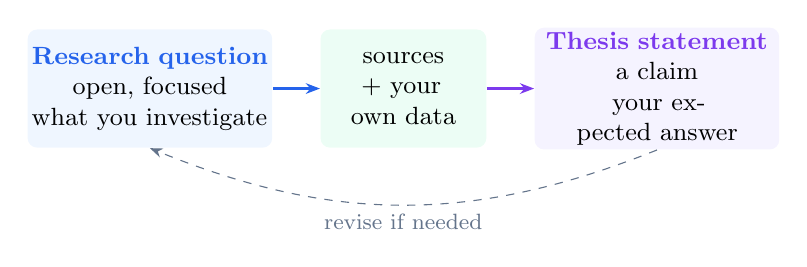
\begin{tikzpicture}[x=1mm,y=1mm,font=\small,
  bx/.style={rounded corners=1.2mm,minimum height=15mm,text width=30mm,align=center,inner sep=1.5pt}]
  \node[bx,fill=primtint] (q) at (0,0) {\textbf{\textcolor{prim}{Research question}}\\open, focused\\what you investigate};
  \node[bx,fill=goodtint,right=6mm of q,text width=20mm] (d) {sources\\+ your own data};
  \node[bx,fill=sectint,right=6mm of d] (t) {\textbf{\textcolor{sec}{Thesis statement}}\\a claim\\your expected answer};
  \draw[-{Stealth[length=1.8mm]},prim,line width=0.8pt] (q) -- (d);
  \draw[-{Stealth[length=1.8mm]},sec,line width=0.8pt] (d) -- (t);
  \draw[-{Stealth[length=1.6mm]},muted,dashed] (t.south) to[bend left=22] node[below,font=\footnotesize,text=muted]{revise if needed} (q.south);
\end{tikzpicture}
\end{minipage}\hfill
\begin{minipage}[t]{0.39\linewidth}\vspace{0pt}
{\small\textbf{Now:} a \emph{working thesis} – for an experiment or survey your \emph{hypothesis}.\par\vspace{0.5mm}
\textbf{End of 12/1:} question fixed.\par\vspace{0.5mm}
\textbf{Final paper:} thesis backed by your results.}
\end{minipage}
\par\vspace{0.5mm}
\kl{In your own words: how do question and thesis work together?}
\lsglinien{2}{The question says what I want to find out; the thesis is my expected answer – a claim that sources and my own data can confirm or prove wrong. If the data disagree, I revise the thesis.}
\end{wsbox}

% ------------------------------------------------------------------ 2
\begin{wsbox}{2}{Six markers of a good research question}
\begin{minipage}[t]{0.5\linewidth}\vspace{0pt}\small
\kl{Focused}\enspace Who or what exactly? Where, when?\par\vspace{0.6mm}
\kl{Open}\enspace no one-search answer, no plain yes/no, no built-in answer\par\vspace{0.6mm}
\kl{Researchable}\enspace Are there sources to build on?
\end{minipage}\hfill
\begin{minipage}[t]{0.47\linewidth}\vspace{0pt}\small
\kl{Testable}\enspace Can I collect my own data?\par\vspace{0.6mm}
\kl{Feasible}\enspace 10–15 pages? Time, access, ethics?\par\vspace{0.6mm}
\kl{Relevant}\enspace So what? And is it about time?
\end{minipage}
\par\vspace{0.5mm}
{\footnotesize\textcolor{muted}{Open question words: \emph{How … / To what extent … / In what ways … / Why …}}}
\end{wsbox}

% ------------------------------------------------------------------ 3
\begin{wsbox}{3}{Spot the problem}
{\small Which marker does each question miss most? Then improve one of them.}\par\vspace{1mm}
\renewcommand{\arraystretch}{1}
\begin{tabularx}{\linewidth}{@{}X p{42mm}@{}}
\arrayrulecolor{rule}\toprule
\textbf{question} & \textbf{missing marker}\\\midrule
\schreibzeile a)\enspace What is the Mayan calendar? & \lsgtext{Open (one search answers it)}\\\midrule
\schreibzeile b)\enspace How does time affect people? & \lsgtext{Focused (who? which effect?)}\\\midrule
\schreibzeile c)\enspace Will humans ever travel back in time? & \lsgtext{Testable (no own data possible)}\\\midrule
\schreibzeile d)\enspace How did all English novels of the 20th century deal with time? & \lsgtext{Feasible (far too much material)}\\\bottomrule
\end{tabularx}
\par\vspace{1mm}
\kl{My improved version of}\enspace\lsg[12mm]{b)}\,:
\lsglinien{2}{How do Year 12 students' estimates of a 10-minute break differ when they spend it on their phones or talking to friends?}
\end{wsbox}

% ------------------------------------------------------------------ 4
\begin{wsbox}{4}{From question to thesis}
\begin{minipage}[t]{0.42\linewidth}\vspace{0pt}
\kl{A thesis statement …}
\begin{itemize}[itemsep=0.2mm]
\item \textbf{answers} the question directly
\item is \textbf{arguable} – not a fact, not a taste
\item is \textbf{specific} – group, material, direction
\item is \textbf{testable} – a result could prove it wrong
\item is \textbf{short} – one or two sentences
\end{itemize}
\end{minipage}\hfill
\begin{minipage}[t]{0.55\linewidth}\vspace{0pt}
{\small\textbf{Question:} To what extent does checking a phone during homework change how long students think they worked?}\par\vspace{0.5mm}
\kl{Your working thesis:}
\lsglinien{3}{Students who check their phones during homework think they worked longer than they actually did – their estimate is further off than that of students without a phone.}
\end{minipage}
\end{wsbox}

% ================================================================== page 2
\newpage

% ------------------------------------------------------------------ 5
\begin{wsbox}{5}{Work phase: read to orient \enspace{\normalfont\small\textcolor{muted}{10 min · aim for 1–3 options by the end of today}}}
\begin{minipage}[t]{0.82\linewidth}\vspace{0pt}
\begin{lueckentext}
My spark: \restzeile
Keywords (English): \restzeile
Names (researchers, authors, works): \restzeile
A debate – where do people disagree? \restzeile
\end{lueckentext}
\end{minipage}\hfill
\begin{minipage}[t]{0.15\linewidth}\vspace{0pt}\raggedleft
\qrcode[height=17mm]{\website}\par
{\scriptsize\textcolor{muted}{strategies + builder}}
\end{minipage}
\end{wsbox}

% ------------------------------------------------------------------ 6
\begin{wsbox}{6}{Question storm \enspace{\normalfont\small\textcolor{muted}{5 min · at least 10 questions · no judging · then mark O (open) / C (closed) and star your best three}}}
\linien{4}
\end{wsbox}

% ------------------------------------------------------------------ 7
\begin{wsbox}{7}{My options}
\renewcommand{\arraystretch}{1}
\begin{tabularx}{\linewidth}{@{}c X X >{\raggedright\arraybackslash}p{38mm}@{}}
\arrayrulecolor{rule}\toprule
 & \textbf{research question} & \textbf{working thesis} & \textbf{my own data – from whom?}\\\midrule
\rule[-8mm]{0pt}{18mm}\headfont\textcolor{prim}{1} & & & \\\midrule
\rule[-8mm]{0pt}{18mm}\headfont\textcolor{prim}{2} & & & \\\midrule
\rule[-8mm]{0pt}{18mm}\headfont\textcolor{prim}{3} & & & \\\bottomrule
\end{tabularx}
\end{wsbox}

% ------------------------------------------------------------------ 8
\begin{wsbox}{8}{Draw the line – for your strongest option}
\begin{minipage}[t]{0.485\linewidth}\vspace{0pt}
\klc{good}{In}\enspace{\footnotesize\textcolor{muted}{material · people · time span · aspect · method}}
\linien{3}
\end{minipage}\hfill
\begin{minipage}[t]{0.485\linewidth}\vspace{0pt}
\klc{bad}{Out – on purpose}
\linien{3}
\end{minipage}
\par\vspace{1mm}
\begin{lueckentext}
This paper focuses on \restzeile
It does not \restzeile
\end{lueckentext}
\end{wsbox}

% ------------------------------------------------------------------ 9
\begin{wsbox}{9}{Partner check}
\begin{minipage}[t]{0.5\linewidth}\vspace{0pt}
{\small
\cb So what – who would want to know?\par\vspace{0.4mm}
\cb What exactly will you collect, from whom?\par\vspace{0.4mm}
\cb Which result would prove your thesis wrong?\par\vspace{0.4mm}
\cb Too big, too small – or right for 10–15 pages?}
\end{minipage}\hfill
\begin{minipage}[t]{0.47\linewidth}\vspace{0pt}
\kl{My partner's tip · my next step}
\linien{2}
\end{minipage}
\end{wsbox}

\end{document}
